\documentclass[10pt,a4paper]{article}

\usepackage{cvpr}
\usepackage{times}
\usepackage{epsfig}
\usepackage{graphicx}
\usepackage{amsmath}
\usepackage{amssymb}
\usepackage{wrapfig}
\usepackage{subcaption}
\usepackage[breaklinks=true,bookmarks=false]{hyperref}
\usepackage{float}
\cvprfinalcopy

\begin{document}

%%%%%%%%% TITLE
\title{\textsf{Advanced Algorithms project Report}}

\author{Giacomo Fabris\\
University of Trento\\
{\tt\small giacomo.fabris-1@studenti.unitn.it}
}

\maketitle
%\thispagestyle{empty}

\section{Introduction}

%-------------------------------------------------------------------------
Objective of the project is to create a classifier which is able to determine which illness (if any) affects the lungs of a patient, based on their thoracic X-rays images. Illnesses shall be classified in 4 categories: none, bacterial infection, COVID-19, viral infection (non-COVID).

The dataset on which the classifier is trained is composed of about 6000 samples, made of (a) the black-white thoracic X-rays image, 256 pixel wide and high, and (b) a feature vector of 84 entries, extracted from the image.

Performance shall be measured as the average over classes of the sensitivity, i.e. the proportion of samples from a given class correctly identified as such. 

\section{Proposed Method}

I considered the use of neural networks to solve the classification task, performing two main experiments:
\begin{enumerate}
    \item using as input the feature vectors only, I implemented a simple feed-forward neural network;
    \item using as input both the pictures and the feature vectors, I implemented a (small) deep neural network.
\end{enumerate}

\subsection{Feed-forward network on feature vectors}

\begin{wrapfigure}{r}{0.25\textwidth}
    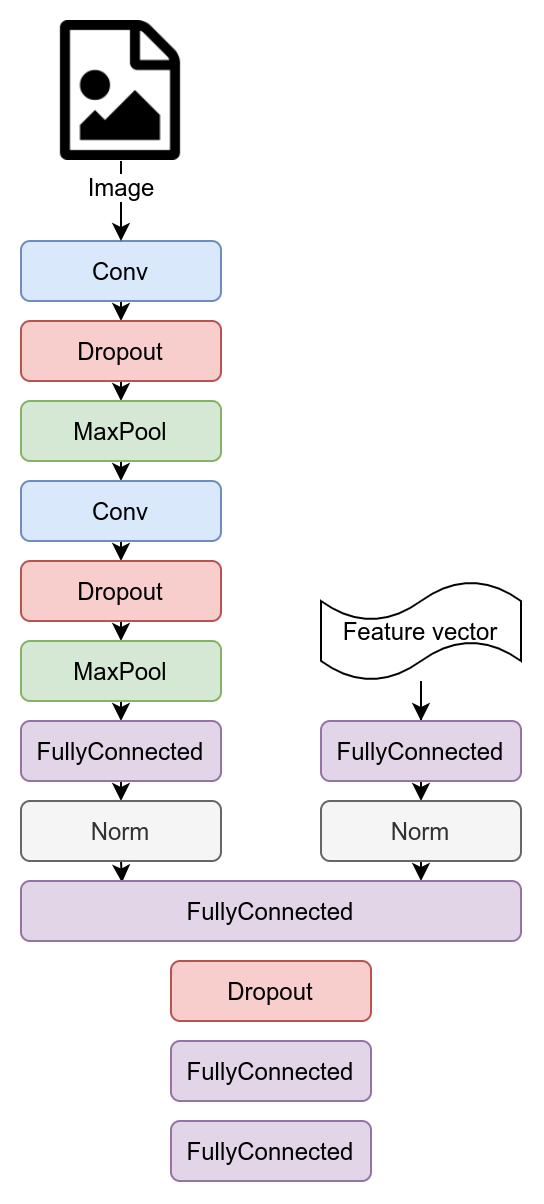
\includegraphics[width=0.9\linewidth]{Network.png}
    \caption{Deep network structure}
\end{wrapfigure}

The feed-forward neural network is composed of 4 layers of, respectively, 84, 42, 21 and 4 perceptron.
Increasing further the number of layers had no sensible effect on the precision of the model; similarly, the effect of changing the number of perceptrons of each hidden layer was not dramatic, above a certain threshold.

I experimented with two optimizers, Stochastic Gradient Descent and Adagrad, and with two activation functions, ReLU and signmoid. The final evaluation has been performed with the Adagrad optimizer, setting an initial learning rate of 5e-4, without weight decay. ReLU has been chosen as activation function. The training has been scheduled using a multi-step learning rate scheduler with a milestone at the 20th epoch; the entire learning lasts 35 epochs. The loss function being used is a weighted cross-entropy loss, where weights compensate the fact that the dataset is not homogeneous in terms of number of instances. For any class $C$ of the dataset $D$, the weight has been set to $1000{|C|}^{-1}$; alternative weights of ${|C|}^{-2}$ and $|C|^{-0.5}$ has been considered but resulted in an unbalanced true positive rate between classes.

%\begin{figure}
%    \centering
%    \subfigure[]{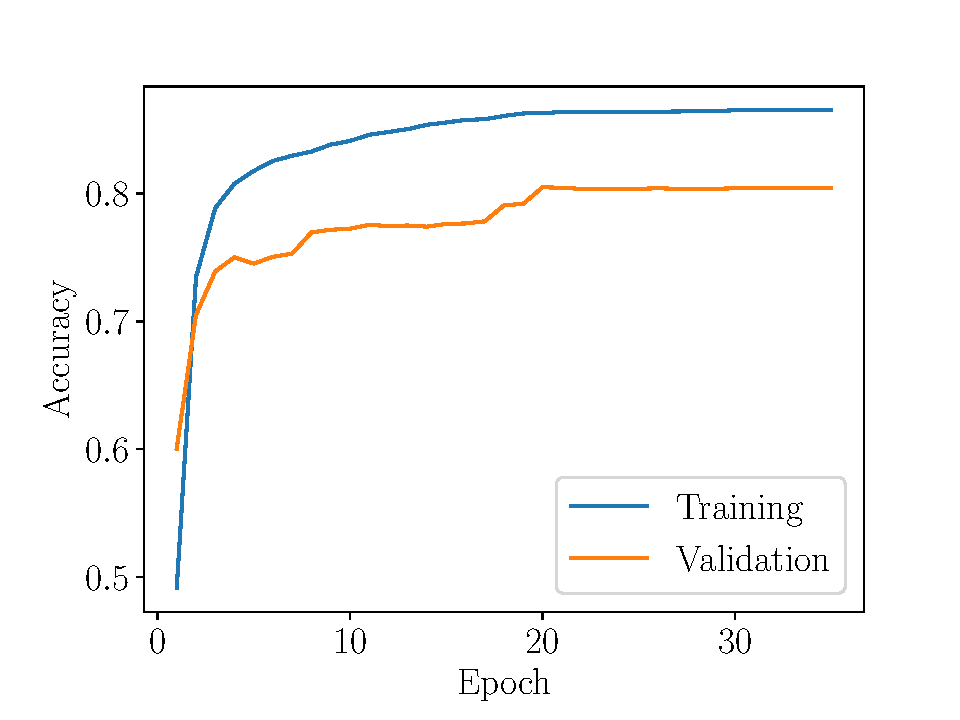
\includegraphics[width=0.45\textwidth]{plot_nn_macc}}
%    \subfigure[]{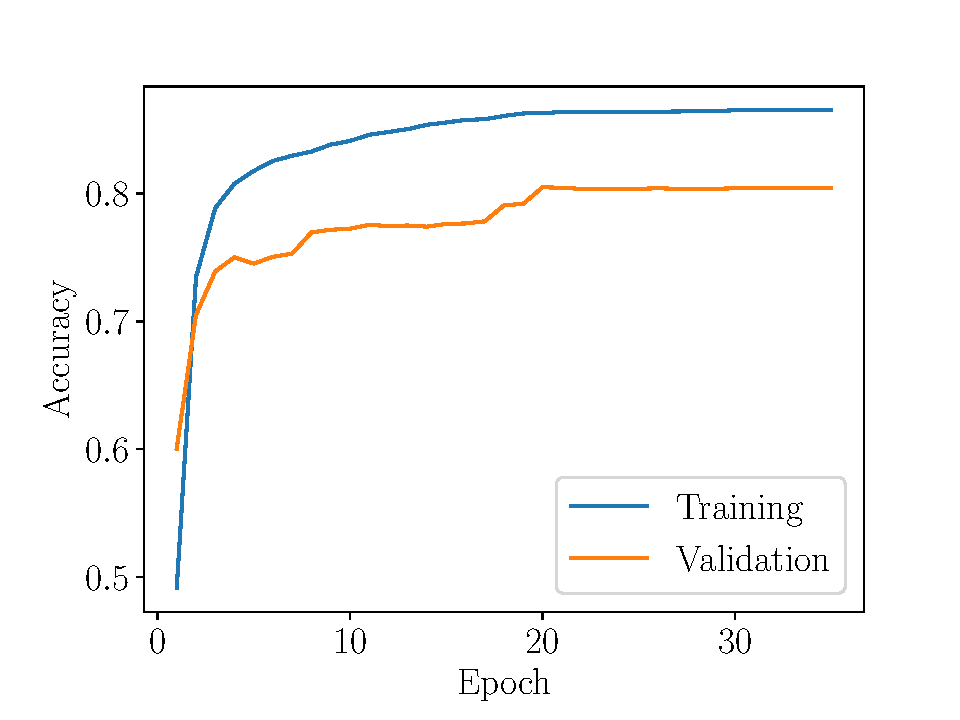
\includegraphics[width=0.45\textwidth]{plot_nn_macc}}
%    \caption{This is the caption}
%\end{figure}

\subsection{Deep network on image dataset}

The deep network is composed of two main segments. The first involves the image processing, and is composed of two main convolution steps, while the second is a feed-forward network which processes the output of the convolution network and the feature vector input. ReLU is chosen as activation function for each step of the network.
Each convolution step is composed of a convolution layer with kernel size 5*5 and stride 1; in order to reduce overfitting, a dropout layer with $p = 0.2$ is inserted after each convolution; then, max pooling with a 3*3 filters is performed to reduce dimensionality.
The output tensor is then linearized and fed into a first layer of perceptrons and normalized, the same processing is performed on the feature vector. Then, the results of the two normalizations are concatenated together into a single vector, which goes through an additional dropout layer with $p = 0.2$ and two perceptron layers.  

As a mean to control overfitting, I considered both dropout layers and weight decays (L2 regolarizers)...

I considered these methods... I noticed these advantages... I noticed these disadvantages ...

The final solution...

\section{Results}

I have implemented the approach with... and performed the following experiments...

%{\small
%\bibliographystyle{ieee}
%\bibliography{egbib}
%}

\end{document}
